\documentclass[12pt]{article}
\usepackage{amsmath}
\usepackage{booktabs}
\usepackage{listings}
\usepackage{graphicx}

\begin{document}

\title{Discrete Assignment-11.9.1-11}
\author{Hiba Muhammed \\
        EE23BTECH11026}
\maketitle

\section*{Problem Statement}
Write the first five terms in the sequence:
\[
\begin{aligned}
a(0)  &= 3 \\
a(n)  &= 3a_{n-1} + 2 \quad \text{for } n > 0
\end{aligned}
\]

\section*{Solution}
\begin{table}[h]
  \centering
  \caption{Input Parameters: First Term and General Formula}
  \begin{tabular}{|c|c|}
    \hline
    \textbf{Term} & \textbf{Value} \\
    \hline
    \(x(0) \) & 3 \\
    \(x(n)\) & \(3x(n-1) + 2\) for \(n > 0\) \\
    \hline
  \end{tabular}
\end{table}
Let's find the first 5 terms of the sequence:
\begin{align}
x(1) &= 3x(0)  + 2 = 3 \times 3 + 2 = 11 \\
x(2) &= 3x(1) + 2 = 3 \times 11 + 2 = 35 \\
x(3) &= 3x(2) + 2 = 3 \times 35 + 2 = 107 \\
x(4) &= 3x(3) + 2 = 3 \times 107 + 2 = 323 \\
x(5) &= 3x(4) + 2 = 3 \times 323 + 2 = 971 
\end{align}

So, the next 5 terms of the sequence are \(11, 35, 107, 323, 971\).



\section*{Solution using Z Transform}
Let's find the Z transform of the sequence \(a(n)\):
\begin{align*}
X(z) &= \mathcal{Z}\{x(n)\} = \sum_{n=0}^{\infty} x(n)z^{-n} \\
&= x(0)z^0 + x(1)z^{-1} + x(2)z^{-2} + x(3)z^{-3} + \ldots \\
&= 3 + (3x(0) + 2)z^{-1} + (3x(1) + 2)z^{-2} + (3x(2) + 2)z^{-3} + \ldots \\
&= 3 + (3 \cdot 3 + 2)z^{-1} + (3 \cdot (3 \cdot 3 + 2) + 2)z^{-2} + (3 \cdot (3 \cdot (3 \cdot 3 + 2) + 2) + 2)z^{-3} + \ldots \\
&= 3 + 11z^{-1} + 35z^{-2} + 107z^{-3} + \ldots
\end{align*}

So, the Z transform of the sequence \(x(n)\) is given by \(X(z) = 3 + 11z^{-1} + 35z^{-2} + 107z^{-3} + \ldots\).

\begin{figure}[h]
    \centering
    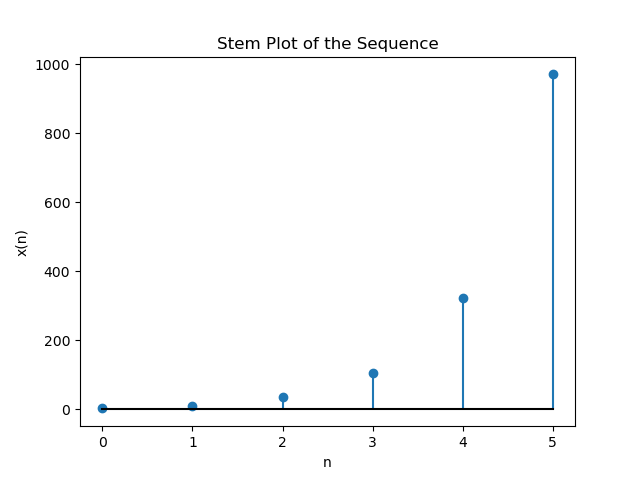
\includegraphics[width=0.7\linewidth]{11.9.1-11.png}
    \caption{Sequence plot generated from Python script.}
    \label{fig:sequence-plot}
\end{figure}

\end{document}

